\section{Field Study}

	The field study took place during the first two weeks of March, from 3/3/2015 to 3/15/2015 in a faculty building of Ludwig-Maximilians-University of Munich. Data was collected on 14 consecutive days and personal semi-structured interviews were carried out on five working days during the same two weeks. A total of 118 interactions were registered with the application installed on the public display and 58 survey responses were recorded.

	The goal of this study was to validate the previous thoughts, get better insights into our research questions, and to see how users respond to questionnaires being conducted on displays in the public.



\subsection{Research Questions}

	One of the main reasons why we performed this field study was to get a better understanding of our assumptions and hypotheses. Especially since there is often a discrepancy between what one assumes and what can actually be observed, as has been stated in the publication by Ojala and Kostakos in 2011: ``Introduction A common criticism targeted at many studies on interactive public displays is that their evaluation usually takes place in non-realistic lab environments, and for short periods of time. Thus, a long-term real- world deployment could be a more appropriate evaluation.''\cite{Ojala2011}.
	% MOTIVATE: explain why we make this field study, explain what we hope to expect. what are our assumptions. what did we expect from the questionnaires, what did we expect from the interviews?

	% Why did we bother to do this study?
		% to find out if our results and predictions validate in the field
	Our assumptions are that we can simplify the conduction and deployment of surveys to public display networks with the help of our PDSurvey platform.

	What do we assume
	What do we want to know
		which variables are there, how do we expect them to change?


	Introduction to the Research Question / How we came to the research question
	\begin{enumerate}
	\item We already had an application running on a public display in a faculty building which attracted lots of regular and new users. Our interest was how we could best integrate questionnaires on and after the application itself (a balloon shooter game).
	\item The first step was to ask ourselves the question, which channel is suited for gathering responses from the audience. ...
	\item Follow up research questions would be: ...
	\end{enumerate}


	The research questions were:

	\begin{itemize}
	\item Which channels are most suited for completing surveys (on a digital platform) in public?
	\item Which question types are best suited for questionnaires carried out in public? What are the requirements in regards to 
	\item In which situations is the user most willing to answer surveys on public displays?
	\item (assessed between the lines) What motivated our users to fill out surveys?
	\item (not really copious): how many questions are acceptable, the attention span would be of great interest
	\item (not really copious): how the users noticed / perceived the survey
	\item (Not treated): where to position the survey on screen. As stated in a paper by J\"org M\"uller ... TODO reference it TODO ..., the best position on large public displays is directly in the center (not at the bottom, not at the top, close to the center). The larger the screen is, the more relevant a centric positioning will get.
	\item (Not treated): How can we best break down a standardized survey with 10+ questions and spread a subset of the questions across multiple users?
	\item (Not treated): The influence of the environment on which question types are suited, how personal the questions can get, how much privacy the display should offer (the smaller, the more private it seems)
	\end{itemize}

	In addition to these questions we were interested in user stories, which feedback they gave us in regards to answering surveys on screens in the public.




\subsection{Study Setup}

	% \paragraph{Participants}
	\subsubsection{Participants}

	\subsubsection{Apparatus}

		Our object of investigation was a large touchscreen with four feedback channels for completing a survey.

		The survey was run on a XXXXX display . The main application installed on the public display was a game called \textit{Balloon Shooter} developed and run by Jiamin Shi, a PhD student at the Group for Media Informatics at LMU Munich.

		\begin{enumerate}
		\item list as detailed information regarding the game as possible
		\item ask Jiamin, whether I can post screenshots of the game?
		\end{enumerate}

	\subsubsection{Location}

	Faculty building for computer science, ethnology, political science, japanologie and physics. m,m

	The study setup was in the entrance hall of the university building, .

	% Show Diagram of User paths inside the entrance hall.


	\subsubsection{Limitations}

	\begin{enumerate}
	\item the tablet was always on, it was possible to approach the tablet directly without having the option to participate in the survey via smartphone or email. 
	\item the novelty effect played a role for the first part of the evaluation. It was striking to see a response rate of 50 percent. If we exclude all participants who directly accessed the tablet and skipped the appeal to use one of the four options, there was still a response rate of 10 percent.
	\end{enumerate}



\subsection{Conditions}

	Feedback channel: 
	\begin{enumerate}
	\item on public display
	\item on tablet, next to the large TV display
	\item via smartphone: 
	\item via email, from home:
	\end{enumerate}


\subsection{Methodology}



\subsection{Quantitative Results}

	\begin{enumerate}
	\item For a good SAMPLE of how to list the basic population (x male, y female) of the survey, have a look at paper number 25 from the Appendix. (WIP)
	\item describe the results from the evaluation
	\item e.g. 1) prefered feedback channel, 2) number of acceptable answers, 3) preferred setting
	\item say which implications this gives for the PDSurvey research platform
	\end{enumerate}

	\begin{enumerate}
	\item Quantitative: pure facts
	\item Qualitative: a combination of facts + evaluation
	\end{enumerate}


	Our primary goal was to find out which channel the users preferred, the questions themselves played a secondary role. The survey displayed on all four channels contained the same five questions. 

	\begin{itemize}
	\item How often have you used this display before? [number]
	\item How likely is it that you will use this display in the future again? [5-point Likert scale]
	\item Which devices do you possess or use regularly? [multiple choice with 5 check boxes]
	\item In which area do you study / work? [text field]
	\item What was your motivation for approaching and using this display? [text field]
	\end{itemize}

	In order to also get first insights into how well certain question types are suited for surveys in public, where a short completion time is crucial, we varied between the following question types and kept them in the same order: numerical question, Likert scale (single click), multiple choice (based on check boxes) and two text fields for an undefinied length of the response. To increase the motivation for participation we stated that the questionnaire consists of five questions, will only take one minute to complete and is for the Master's thesis of student at LMU Munich (see figure \ref{fig:5-pdclient-intro}).
	As proven by Richard Ryan in his self-determination theory\cite{ryan2000self}\footnote{http://www.selfdeterminationtheory.org/}, this additional intrinsic motivation increased the participation and acceptance rate of the public survey additionally. 

	\begin{figure}
	    \begin{center}
	        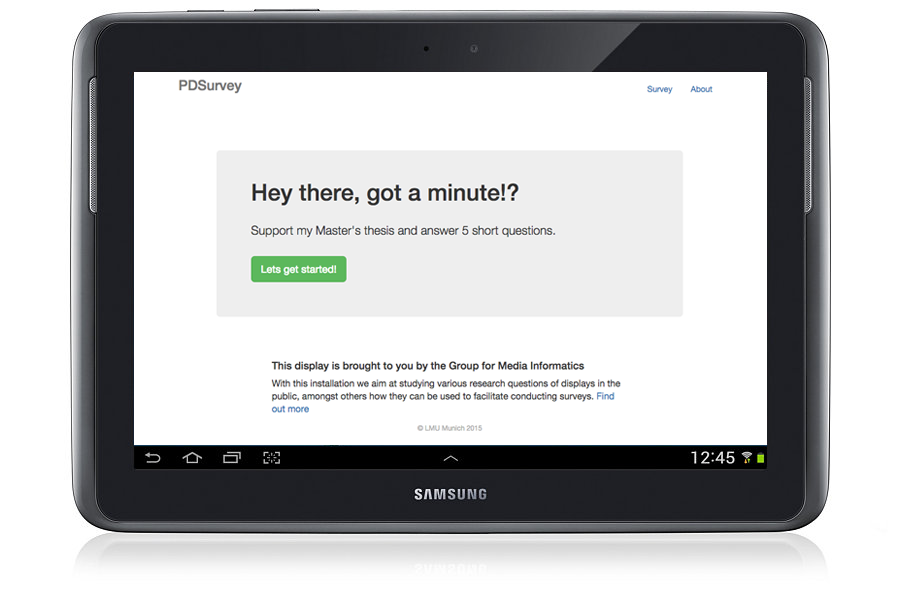
\includegraphics[width=.7\columnwidth]{img/5_field-study/pdclient-startscreen.png}
	    \end{center}
	 \caption{PDClient: Motivating users to participate in a short questionnaire}
	 \label{fig:5-pdclient-intro}
	\end{figure}

	The first question (numeric) was completed in all surveys. 

	To find out more about the motive we carried out semi-structured interviews on location.


\subsection{Qualitative Results}




\subsection{Discussion AND/OR Summary}

	Start with a few sentences that summarize the most important results (+ see \url{http://www.ldeo.columbia.edu/~martins/sen_sem/thesis_org.html}).

	Now allowing room for interpretation and personal opinions

	\begin{enumerate}
	\item (summarize the expert interviews)
	\item summarize the quantitative results
	\item summarize the qualitative results 
	\item TODO: think about what my evaluation has to do with my platform. make sure that this link is clear! Make this link clear in the following summary.
	\end{enumerate}

